% Protocol architecture as measured in this study (Fig. 1).
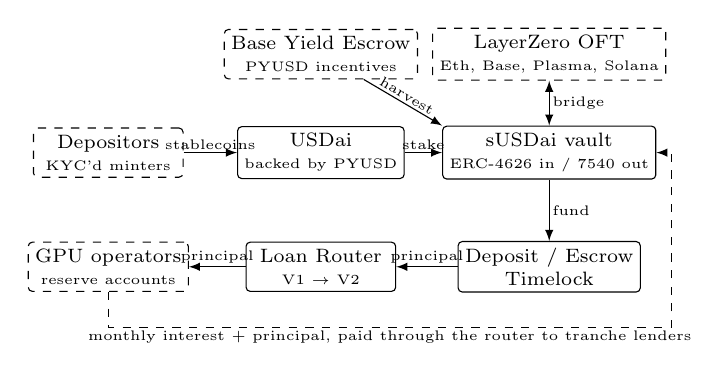
\begin{tikzpicture}[
  font=\scriptsize, >=latex,
  box/.style={draw, rounded corners=1.5pt, align=center, inner sep=2.5pt, minimum height=6mm, minimum width=19mm, fill=white},
  ext/.style={box, dashed},
  lab/.style={font=\tiny, align=center, inner sep=1pt}]
  % row 1
  \node[ext] (dep)   at (0,0)    {Depositors\\{\tiny KYC'd minters}};
  \node[box] (usdai) at (2.7,0)  {USDai\\{\tiny backed by PYUSD}};
  \node[box] (vault) at (5.6,0)  {sUSDai vault\\{\tiny ERC-4626 in / 7540 out}};
  \node[ext] (lz)    at (5.6,1.25) {LayerZero OFT\\{\tiny Eth, Base, Plasma, Solana}};
  \node[ext] (bye)   at (2.7,1.25) {Base Yield Escrow\\{\tiny PYUSD incentives}};
  % row 2
  \node[box] (dt)    at (5.6,-1.45) {Deposit / Escrow\\Timelock};
  \node[box] (lr)    at (2.7,-1.45) {Loan Router\\{\tiny V1 $\rightarrow$ V2}};
  \node[ext] (bor)   at (0,-1.45)   {GPU operators\\{\tiny reserve accounts}};
  % flows
  \draw[->] (dep) -- node[lab, above] {stablecoins} (usdai);
  \draw[->] (usdai) -- node[lab, above] {stake} (vault);
  \draw[<->] (vault) -- node[lab, right] {bridge} (lz);
  \draw[->] (bye) -- node[lab, above, sloped] {harvest} (vault.north west);
  \draw[->] (vault) -- node[lab, right] {fund} (dt);
  \draw[->] (dt) -- node[lab, above] {principal} (lr);
  \draw[->] (lr) -- node[lab, above] {principal} (bor);
  \draw[->, dashed] (bor.south) -- ++(0,-0.45) -- node[lab, below] {monthly interest + principal, paid through the router to tranche lenders} ++(7.15,0) |- (vault.east);
\end{tikzpicture}
